\chapter{Anexo}
	
\section{Manual}
	
Tras compilar el repositorio o haber descargado un ejecutable, es preciso incluir en la línea de comandos tres parámetros. El primero es el directorio donde se encuentra la escena, el segundo es el número de muestras deseado y el tercero el archivo de salida en formato .bmp de la imagen resultante.
	
\subsection{Formato de escenas}
\label{sceneformat}

Debido a la falta de consenso en cuanto a formatos en la industria, se ha utilizado un formato de escenas intentando respetar los estándares más comunes. Así pues una escena se define como un directorio.

Dentro este directorio debe incluir en su interior 3 carpetas

\begin{itemize}
	\item Objects: utilizada para las geometrías en formato .obj. Es necesario que estas geometrías hayan sido trianguladas previamente puesto que el parser desarrollado está limitado a triángulos.
	
	\item Textures: utilizada para las texturas. Actualmente solo se permiten texturas para los atributos: Albedo, Emission, Roughness, Metallic, Normal. Las texturas tienen que estar en formato bmp de 24 bits. El formato de nombre es el siguiente: nombredelmaterial\_tipodemapa.bmp. Por ejemplo: material1\_albedo.bmp, material1\_metallic.bmp. No es necesario que se definan todas las texturas, si no existe alguna se ignorará y se utilizará el valor de color definido en el archivo scene.json. En caso de no existir tampoco ese valor, se utilizará el valor por defecto. Las texturas de albedo y emisión deberán encontrarse en espacio de color sRGB mientras que el resto de texturas deben estar en un espacio lineal. Esto no es respetado por muchos motores de renderizado y es dependiente de la implementación.
	
	\item HDRI: utilizada para los mapas de entorno. Dentro albergará los archivos en formato .hdr de los mapas de entorno.
\end{itemize}

Además será obligatorio incluir un archivo llamado scene.json. Este archivo ha de incluir la información de la escena necesaria. Se muestra un ejemplo como plantilla:

\begin{lstlisting}
	
{	
'camera' : {'xRes' : 1280, 'yRes' : 720, 'position' : {x : 0, y : 1, z : 2}, 'focalLength' : 0.05, 'focusDistance' : 1, 'aperture' : 2.8},
'materials' : [{'name' : 'mat1'}, {'name' : 'mat2', 'albedo' : {'r' : 1, 'g' : 0, 'b' : 0}, 'roughness' : 0.2}],
'objects' : [{'name' : 'obj1', 'material' : 'mat1'}, {'name' : 'obj2', 'material' : 'mat2'}],
'hdri' : {'name' : 'hdri', 'xOffset' : 0.5},
}
	
\end{lstlisting}

El ejemplo mostrado deberá contener dos objetos dentro de la carpeta Objects: obj1.obj y obj2.obj. El material mat1 utilizará las texturas que empiecen por mat1\_...bmp mientras que el mat2 utilizará los valores rgb(1,0,0) para albedo y el valor 0.2 para roughness. Para más ejemplos consultar la carpeta Scenes del repositorio.

\subsection{Ejemplo de renderizado de escena \emph{ClockCC0}}

Con el fin de demostrar el funcionamiento con un ejemplo real, se ha preparado una escena para la cual, todos los recursos tienen licencia CC0. Esta escena se encuentra en el repositorio y puede ser recreada si se siguen los pasos mostrados en este punto.

Los modelos y texturas utilizados para esta escena son los siguientes:

\begin{itemize}
	\item Modelo de planta: \url{https://polyhaven.com/a/potted_plant_04}
	\item Modelo de mesa: \url{https://polyhaven.com/a/vintage_wooden_drawer_01}
	\item Modelo de reloj: \url{https://polyhaven.com/a/alarm_clock_01}
	\item HDRI de interior: \url{https://polyhaven.com/a/photo_studio_london_hall}
\end{itemize}

Para la ejecución del programa, en el entorno utilizado, ha sido necesario utilizar los siguientes argumentos:
	\code{eleven.exe ''C:$\backslash\backslash$Users$\backslash\backslash$Kike$\backslash\backslash$Desktop$\backslash\backslash$Uni$\backslash\backslash$TFG$\backslash\backslash$Scenes$\backslash\backslash$ClockCC0'' output.bmp 5000}

Tras comenzar el renderizado aparecen dos ventanas, la primera es la consola de salida que se muestra en la \autoref{fig:debugwindow}. Esta ventana contiene datos relevantes en cuanto a la ejecución, como: El progreso de la construcción del BVH, cantidad de memoria utilizada por las geometrías/texturas, eficiencia en kPaths/s, cuanta memoria consume la escena en la GPU y cuanta hay libre, cuantas muestras se han tomado y el tiempo total de ejecución.

Por otro lado, está la ventana de previsualización \autoref{execsamples}. Esta ventana muestra el progreso visual del render y en la esquina superior izqda, el número de muestras tomadas por cada pixel hasta el momento.

Finalmente la imagen será guardada como "render.bmp" tras ejecutar las 5000 muestras. En este caso la salida es la \autoref{fig:finalimagewindow}. Este resultado se ha obtenido tras 20 minutos y 39 segundos en una NVIDIA RTX 3090. Con un número mucho menor de muestras es posible seguir obteniendo buenos resultados.

\begin{figure}[H]
    \centering
	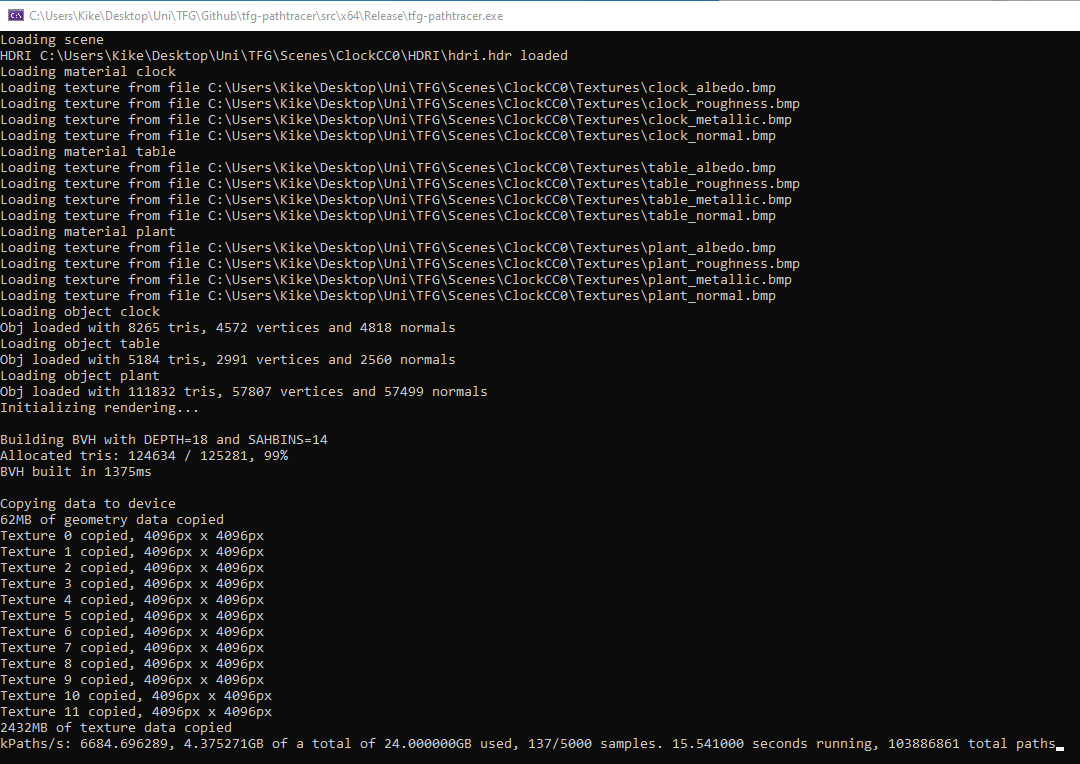
\includegraphics[width=0.9\textwidth]{execdebug}
	\caption{Ventana de depuración}
	\label{fig:debugwindow}
\end{figure}

\begin{figure}[H]
    \centering
	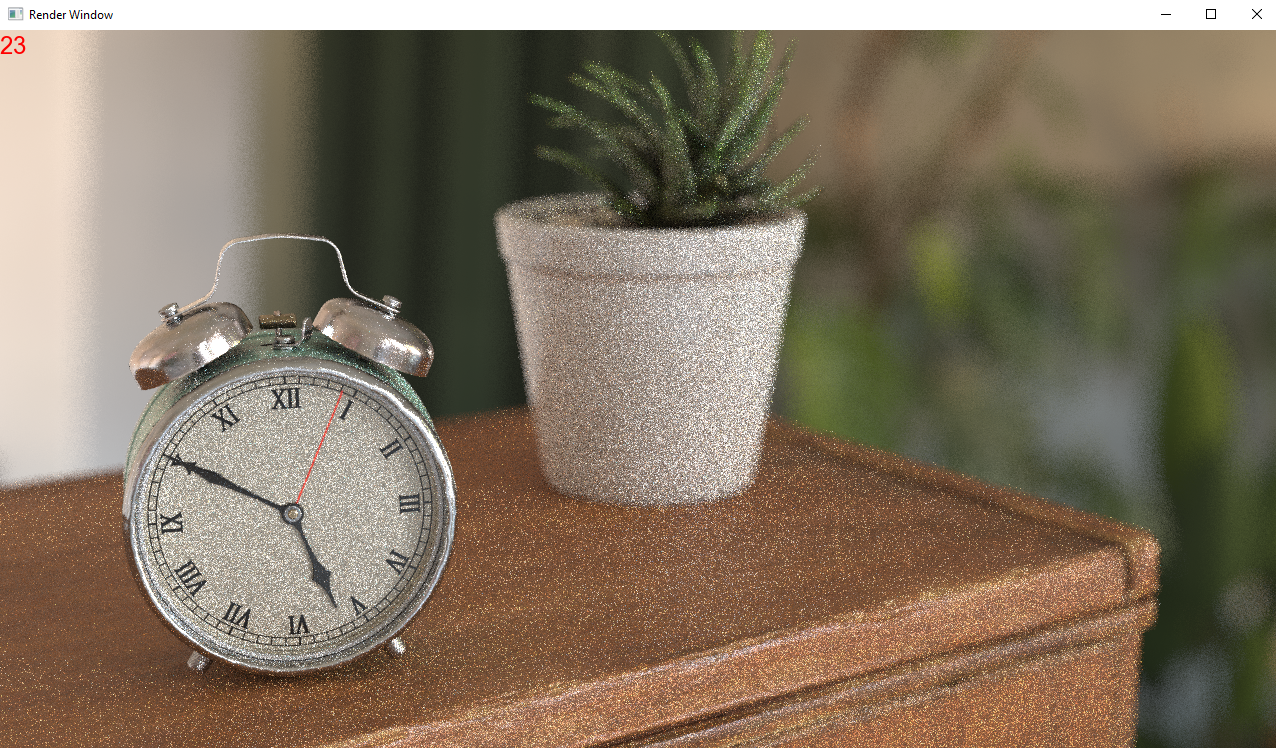
\includegraphics[width=0.9\textwidth]{execsamples}
	\caption{Ventana de previsualización}
	\label{fig:samplewindow}
\end{figure}

\begin{figure}[H]
    \centering
	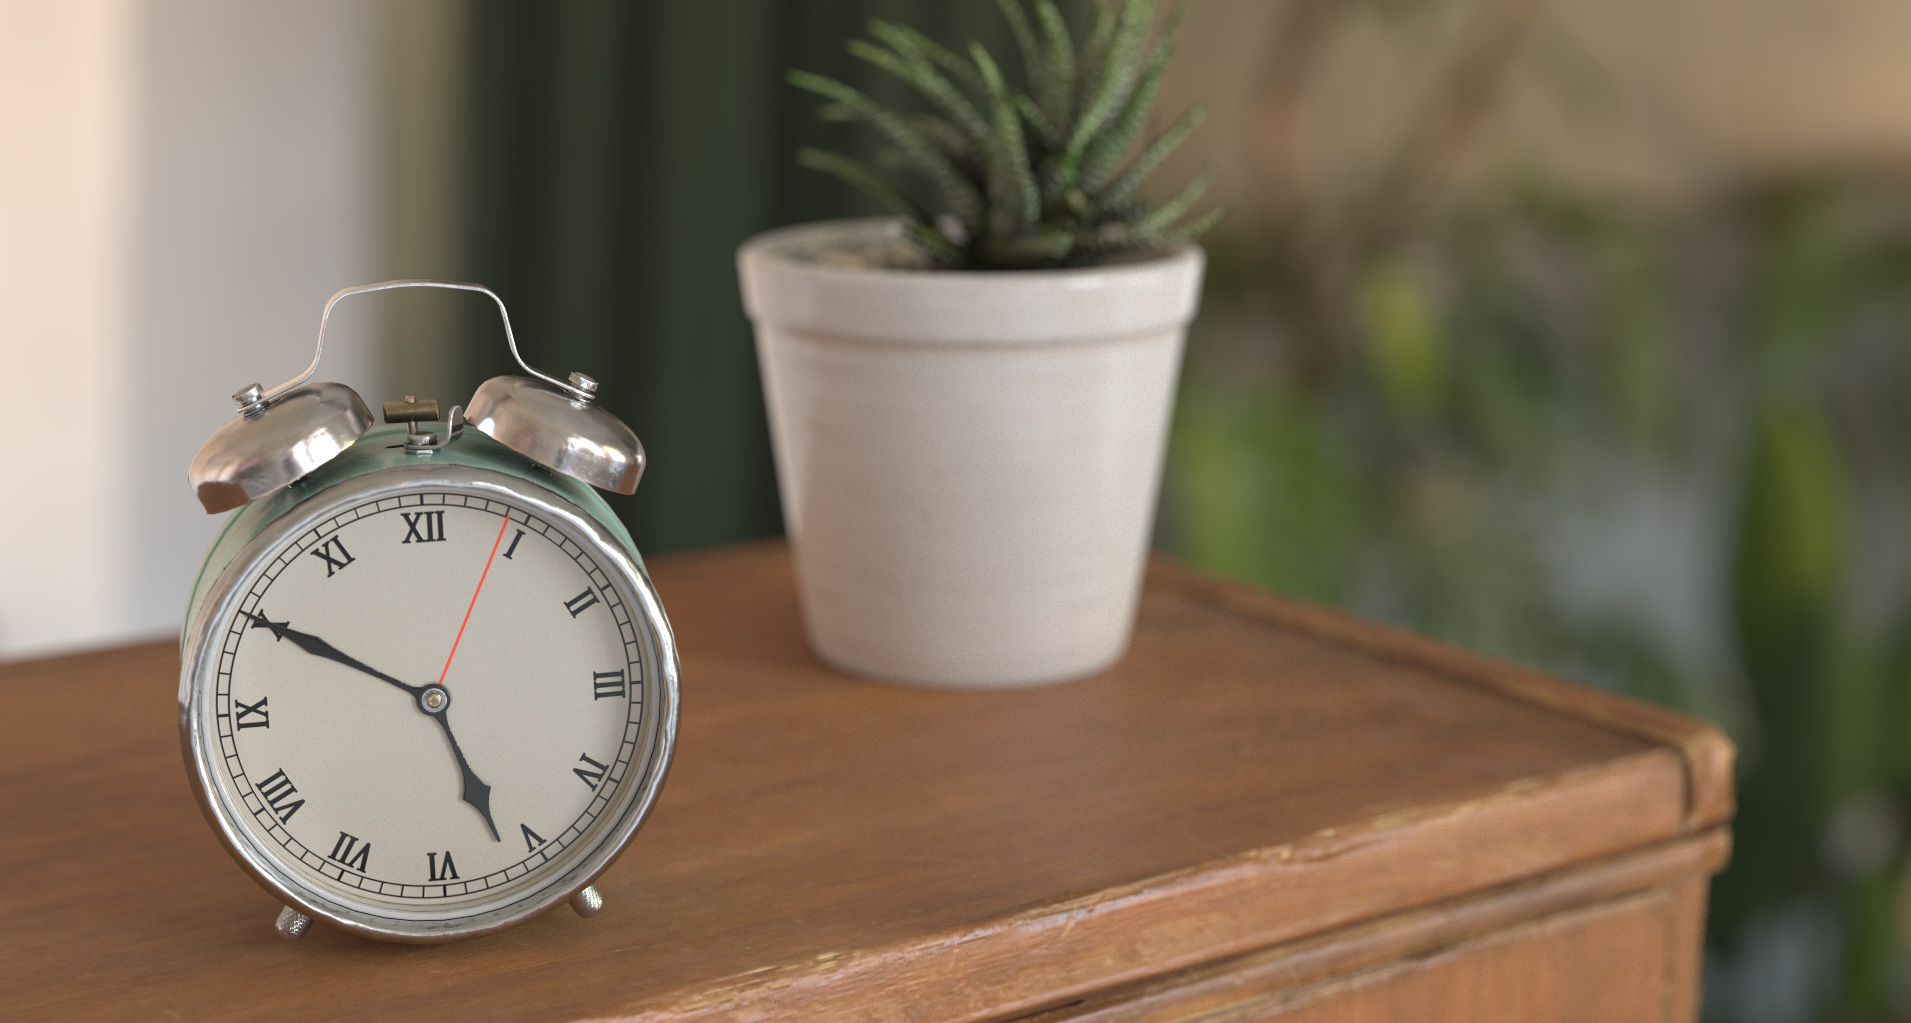
\includegraphics[width=0.9\textwidth]{execfinalimage}
	\caption{Ventana de previsualización}
	\label{fig:finalimagewindow}
\end{figure}

\section{Galería}
	